 \documentclass[25 pt,margin=0.9in,innermargin=-4.5in,blockverticalspace=-0.25in]{tikzposter}
\geometry{paperwidth=43in,paperheight=32.5in}
\usepackage[utf8]{inputenc}
\usepackage{amsmath}
\usepackage{amsfonts}
\usepackage{amsthm}
\usepackage{amssymb}
\usepackage{mathrsfs}
\usepackage{graphicx}
\usepackage{adjustbox}
\usepackage{enumitem}
\usepackage{wrapfig}
\usepackage{mwe} % for placeholder images
\usepackage{comment}
\usepackage[backend=biber,style=numeric]{biblatex}
\usepackage{SUtheme}

%tikz
\usepackage{tikz}
\usetikzlibrary{arrows.meta,decorations.markings}
\tikzset{
  ->-/.style={decoration={
    markings,
    mark=at position #1 with {\arrow{>}}},
    postaction={decorate}}
}
\usetikzlibrary{calc}


\addbibresource{refs.bib}

% set theme parameters
\tikzposterlatexaffectionproofoff
\usetheme{SUTheme}
\usecolorstyle{SUStyle}
\usetitlestyle{Filled}

\usepackage[scaled]{helvet}
\renewcommand\familydefault{\sfdefault} 
\usepackage[T1]{fontenc}

\linespread{0.9}

\title{Braid your Braid Group Representations}
%\author{Zih-Yu Hsieh \quad \quad Mentor: Choomno Moos}
\institute{UC Santa Barbara, College of Creative Studies}
\titlegraphic{\includegraphics[width=0.06\textwidth]{logo.png}}

% begin document
\begin{document}
\maketitle
\centering
\begin{columns}
    \column{0.30}
    \block{What's a Braid Group?}{
        \textbf{Def:} $n$-strand \emph{Braid Group} $B_n$ is generated by $\{\sigma_1,...,\sigma_{n-1}\}$, satisfying \textbf{Braid Relations}: 
        \begin{center}
            $\sigma_i \sigma_j = \sigma_j \sigma_i$ if $|i-j|\geq 2$; $\quad\quad$ $\sigma_i \sigma_{i+1}\sigma_i = \sigma_{i+1}\sigma_i \sigma_{i+1}$
        \end{center}
        \vspace{-0.5em}
        \begin{tikzfigure}
            \centering
            \includegraphics[width=0.3\linewidth]{braid diagrams 2.jpg}
        \end{tikzfigure}
        \begin{center}
            \textbf{Figure:} Geometric Braid of $4$ strands
        \end{center}

        %https://www.science.org/doi/10.1126/science.1231473 image source
    }

    \block{$B_n$ as Mapping Class Groups}{ 
        \textbf{Def:} Let $D_n$ be an $n$-punctured disk. Its \emph{Mapping Class Group} $\mathfrak{M}(D_n)$ collects isotopic classes of self-homeomorphisms that fixes disk boundary $\partial D$.

        \textbf{Ex:} The $i^\textmd{th}$ \emph{Half Twist} $\tau_i \in \mathfrak{M}(D_n)$ swaps $i^\textmd{th}$, $(i+1)^\textmd{th}$ punctures.

        \begin{center}
            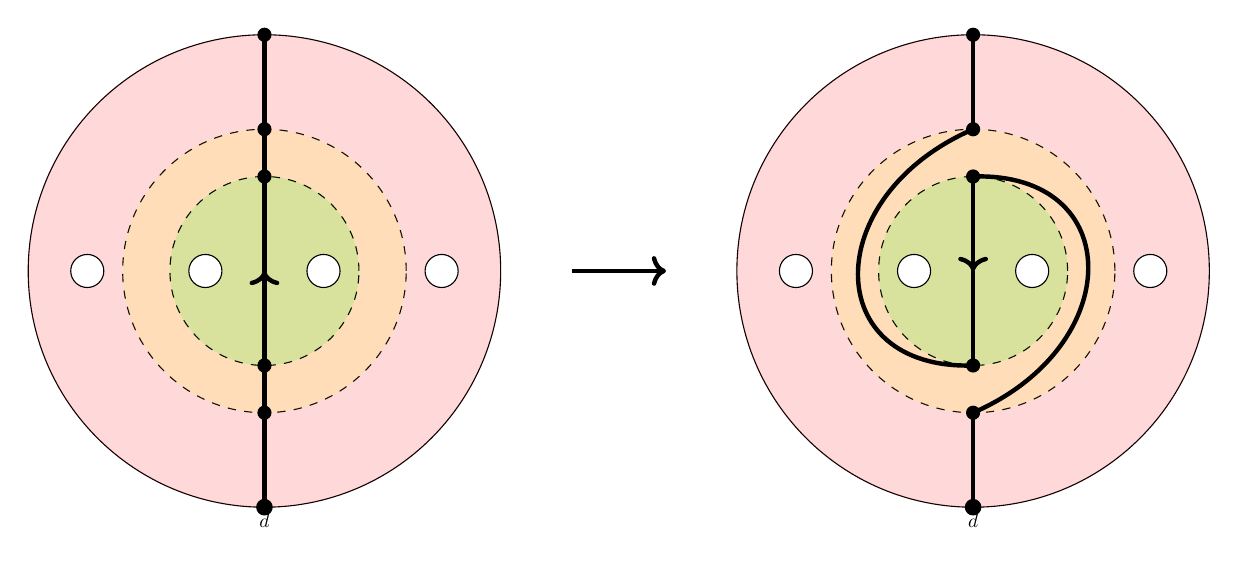
\begin{tikzpicture}[scale=3]
                %Left: original punctured disk
                % Large most circle
                \draw (0,0) circle (1); % big circle
                \fill[red,opacity=0.15] (0,0) circle (1);

                %middle circle
                \draw[dashed] (0,0) circle (0.6);
                \fill[yellow, opacity=0.15] (0,0) circle (0.6);

                %small circle
                \draw[dashed] (0,0) circle (0.4);
                \fill[green, opacity=0.15] (0,0) circle (0.4);

                %indication line
                \draw[ultra thick] (0,0.4) -- (0,1);
                \draw[ultra thick] (0,-1) -- (0,-0.4);
                \draw[ultra thick, ->-=0.5] (0,-0.4) -- (0,0.4);

                %dots along indication arrow
                \foreach \y in {-0.6,-0.4,0.4,0.6,1}
                    \fill[black] (0,\y) circle (0.03);
                
                % Basepoint
                \fill (0,-1) circle (1pt) node[below, scale=0.7] {$d$};
                
                % Punctures
                \foreach \x in {-0.75, -0.25, 0.25, 0.75}
                    \fill[white] (\x,0) circle (0.07);
                \foreach \x in {-0.75, -0.25, 0.25, 0.75}
                    \draw (\x,0) circle (0.07);


                %mapping arrows
                \draw[->, ultra thick] (1.3,0) -- (1.7,0);


                %Right: twisted punctured disk (everything except the arrow, shifted by x+3
                % Large most circle
                \draw (3,0) circle (1); % big circle
                \fill[red,opacity=0.15] (3,0) circle (1);

                %middle circle
                \draw[dashed] (3,0) circle (0.6);
                \fill[yellow, opacity=0.15] (3,0) circle (0.6);

                %small circle
                \draw[dashed] (3,0) circle (0.4);
                \fill[green, opacity=0.15] (3,0) circle (0.4);

                %indication arrow
                \draw[ultra thick,->-=0.5] (3,0.4) -- (3,-0.4);
                \draw[ultra thick] (3,-1) -- (3,-0.6);
                \draw[ultra thick] (3,0.6) -- (3,1);
                \draw[ultra thick] 
                    (3,-0.4) .. controls (2.35,-0.42) and (2.35,0.318) .. (3,0.6);
                \draw[ultra thick] 
                    (3,0.4) .. controls (3.65,0.42) and (3.65,-0.318) .. (3,-0.6);

                %dots along indication arrow
                \foreach \y in {-0.6,-0.4,0.4,0.6,1}
                   \fill[black] (3,\y) circle (0.03);
                
                % Basepoint
                \fill (3,-1) circle (1pt) node[below, scale=0.7] {$d$};
                
                % Punctures
                \foreach \x in {2.25, 2.75, 3.25, 3.75}
                    \fill[white] (\x,0) circle (0.07);
                \foreach \x in {2.25, 2.75, 3.25, 3.75}
                    \draw (\x,0) circle (0.07);
            \end{tikzpicture}
            
            \textbf{Figure:} $n=4$, Half Twist $\tau_2$'s Action on $D_4$
        \end{center}

        \textbf{Property:} $B_n\cong \mathfrak{M}(D_n)$, by $\sigma_i \mapsto \tau_i$.
    }

    \block{Braid Automorphism}{
        Fix $d \in \partial D$, the \textbf{Fundamental Group} $\pi_1(D_n, d)\cong F_n$, a \emph{Degree-$n$ Free Group} generated by the $n$ loops.

        \begin{center}
            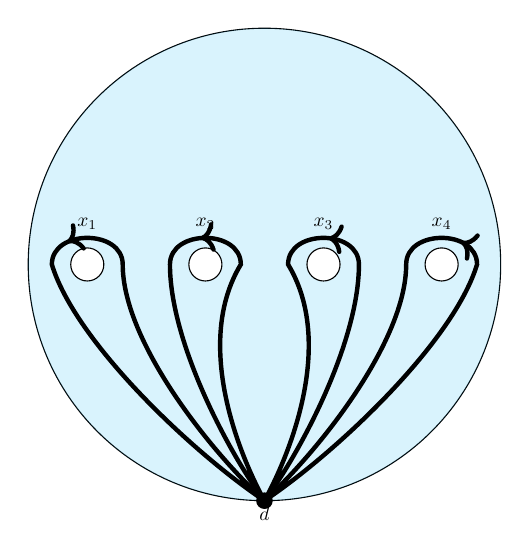
\begin{tikzpicture}[scale=3]
                \draw (0,0) circle (1); % big circle
            
                % Shading inside the disk
                \fill[cyan,opacity=0.15] (0,0) circle (1);
                
                % Basepoint
                \fill (0,-1) circle (1pt) node[below, scale=0.7] {$d$};
                
                % Punctures
                \foreach \x in {-0.75, -0.25, 0.25, 0.75}
                    \fill[white] (\x,0) circle (0.07);
                \foreach \x in {-0.75, -0.25, 0.25, 0.75}
                    \draw (\x,0) circle (0.07);
                
                % Loops from basepoint to punctures
                \draw[->-=0.5, ultra thick] (0,-1) .. controls (-0.22,-0.8) and (-0.6,-0.33) .. (-0.6,0) .. node[above, scale=0.7]{$x_1$} controls (-0.6,0.15) and (-0.9,0.15) .. (-0.9,0) .. controls (-0.8,-0.33) and (-0.3,-0.8) .. (0,-1); %left most
                \draw[ultra thick, ->-=0.5] (0,-1) .. controls (0.3,-0.8) and (0.8,-0.33) .. (0.9,0) .. node[above, scale=0.7]{$x_4$} controls (0.9, 0.15) and (0.6, 0.15) .. (0.6,0) .. controls (0.6, -0.33) and (0.22,-0.8) .. (0,-1); %right most (mirror of left most)
                \draw[->-=0.5, ultra thick] (0,-1) .. controls (-0.11,-0.8) and (-0.3,-0.33) .. (-0.1,0) .. node[above, scale=0.7]{$x_2$} controls (-0.1,0.15) and (-0.4,0.15) .. (-0.4,0) .. controls (-0.4,-0.33) and (-0.15,-0.8) .. (0,-1); %middle left
                \draw[ultra thick, ->-=0.5] (0,-1) .. controls (0.15,-0.8) and (0.4,-0.33) .. (0.4,0) .. node[above, scale=0.7]{$x_3$} controls (0.4,0.15) and (0.1,0.15) .. (0.1,0) .. controls (0.3,-0.33) and (0.11,-0.8) .. (0,-1); %middle right (mirror of middle left)
            \end{tikzpicture}

            \textbf{Figure:} Loops Generating $\pi_1(D_4,d)$
        \end{center}

        Maps in $\mathfrak{M}(D_n)$ generate \textbf{Braid Automorphisms} on $\pi_1(D_n,d)$.

        \textbf{Ex:} Half Twist's action on $\pi_1(D_n,d)$:
            \[(\tau_i)_*(x_j) = \begin{cases}
            x_{i+1} & j=i\\
            x_{i+1}x_ix_{i+1}^{-1} & j=i+1\\
            x_i & \textmd{Otherwise}
        \end{cases}\]

        \begin{center}
         %(\tau_i)_*\in \mathrm{Aut}(\pi_1(D_n,d)),\quad 
            %try input a braid 
            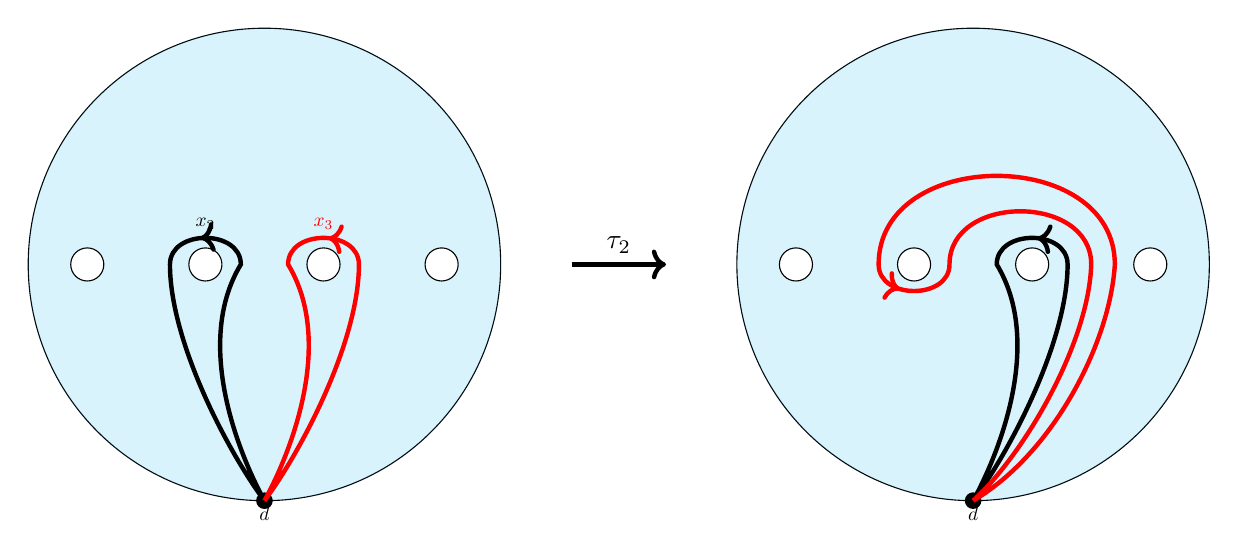
\begin{tikzpicture}[scale=3]
                %left circle, before twisted
                \draw (0,0) circle (1); % big circle
            
                % Shading inside the disk
                \fill[cyan,opacity=0.15] (0,0) circle (1);
                
                % Basepoint
                \fill (0,-1) circle (1pt) node[below, scale=0.7] {$d$};
                
                % Punctures
                \foreach \x in {-0.75, -0.25, 0.25, 0.75}
                    \fill[white] (\x,0) circle (0.07);
                \foreach \x in {-0.75, -0.25, 0.25, 0.75}
                    \draw (\x,0) circle (0.07);
                
                % Loops from basepoint to punctures
                \draw[->-=0.5, ultra thick] (0,-1) .. controls (-0.11,-0.8) and (-0.3,-0.33) .. (-0.1,0) .. node[above, scale=0.7]{$x_2$} controls (-0.1,0.15) and (-0.4,0.15) .. (-0.4,0) .. controls (-0.4,-0.33) and (-0.15,-0.8) .. (0,-1); %middle left
                \draw[red, ultra thick, ->-=0.5] (0,-1) .. controls (0.15,-0.8) and (0.4,-0.33) .. (0.4,0) .. node[above, scale=0.7]{$x_3$} controls (0.4,0.15) and (0.1,0.15) .. (0.1,0) .. controls (0.3,-0.33) and (0.11,-0.8) .. (0,-1); %middle right (mirror of middle left)


                %arrow
                \draw[ultra thick, ->] (1.3,0) -- node[above]{$\tau_2$} (1.7,0);

                
                %right side, twisted 
                \draw (3,0) circle (1); % big circle
            
                % Shading inside the disk
                \fill[cyan,opacity=0.15] (3,0) circle (1);
                
                % Basepoint
                \fill (3,-1) circle (1pt) node[below, scale=0.7] {$d$};
                
                % Punctures
                \foreach \x in {2.25, 2.75, 3.25, 3.75}
                    \fill[white] (\x,0) circle (0.07);
                \foreach \x in {2.25, 2.75, 3.25, 3.75}
                    \draw (\x,0) circle (0.07);
                
                % Loops from basepoint to punctures
                \draw[ultra thick, ->-=0.5] (3,-1) .. controls (3.15,-0.8) and (3.4,-0.33) .. 
                                        (3.4,0) .. controls (3.4,0.15) and (3.1,0.15) .. 
                                        (3.1,0) .. controls (3.3,-0.33) and (3.11,-0.8) .. 
                                        (3,-1); %x_2 sends to x_3

                \draw[red, ultra thick, ->-=0.55] (3,-1) .. controls (3.34,-0.8) and (3.58, -0.33) .. 
                                            (3.6,0) .. controls (3.6, 0.5) and (2.6, 0.5) .. 
                                            (2.6,0) .. controls (2.6, -0.15) and (2.9, -0.15) .. 
                                            (2.9,0) .. controls (2.9, 0.3) and (3.5, 0.3) .. 
                                            (3.5, 0) .. controls (3.49, -0.33) and (3.22, -0.8) .. 
                                            (3, -1);% x_3 sends to x_3 x_2 x_3^{-1}
            \end{tikzpicture}

            \textbf{Figure:} $\tau_2$ Action on $\pi_1(D_4,d)$
        \end{center}
    }
    
    \column{0.40} 

    \block{Reduced Burau Representation}{
        $\psi_n^r:B_n \rightarrow \mathrm{GL}_{n-1}(\mathbb{Z}[t^\pm])$ satisfies:
        $$\sigma_1\mapsto \left(\begin{array}{cc|c}
            -t & 0 & 0 \\
             1 & 1 & 0 \\
             \hline 
             0 & 0 & I_{n-3}
        \end{array}\right),\ \sigma_{n-1}\mapsto \left(\begin{array}{c|cc}
            I_{n-3} & 0 & 0\\
            \hline 
            0 & 1 & t\\
            0 & 0 & -t
        \end{array}\right),\ \sigma_i\mapsto \left(\begin{array}{c|ccc|c}
            I_{i-2} & 0 & 0 & 0 & 0\\
            \hline
            0 & 1 & t & 0 & 0\\
            0 & 0 & -t & 0 & 0\\
            0 & 0 & 1 & 1 & 0\\
            \hline
            0 & 0 & 0 & 0 & I_{n-i-2}
        \end{array}\right)$$
    }

    \block{EX: Burau Representation on $D_4$}{
        $D_4$ \textbf{Continuously Deforms} into $4$ circles join at a point ($\bigvee_{i=1}^4S^1$).

        \begin{center}
            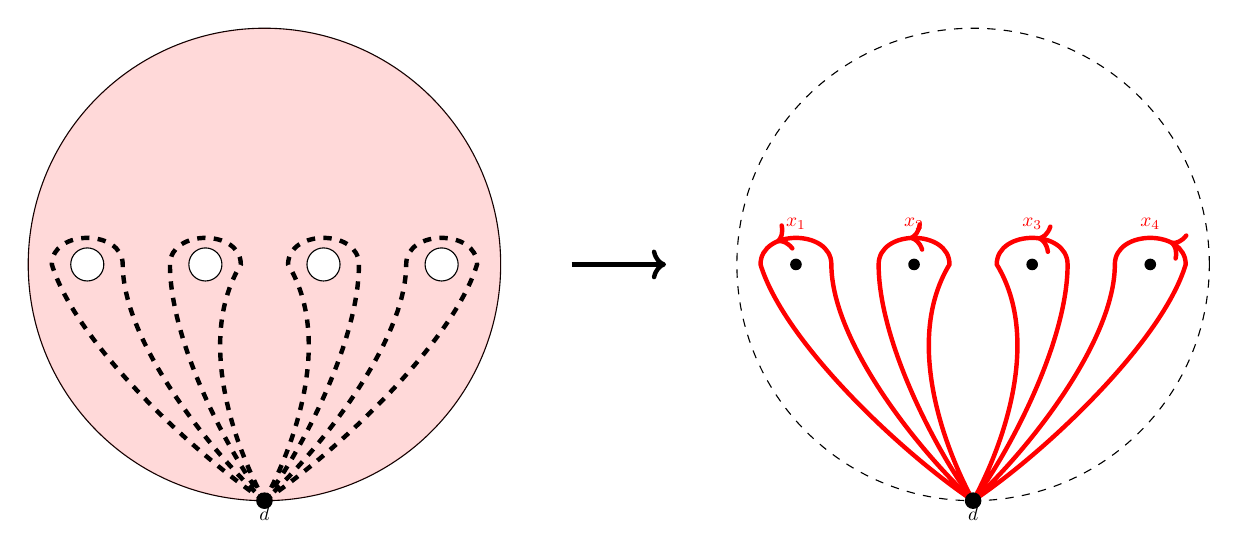
\begin{tikzpicture}[scale=3]
            % Left side: punctured disk
            \draw (0,0) circle (1); % big circle
            
            % Shading inside the disk
            \fill[red,opacity=0.15] (0,0) circle (1);
            
            % Basepoint
            \fill (0,-1) circle (1pt) node[below, scale=0.7] {$d$};
            
            % Punctures
            \foreach \x in {-0.75, -0.25, 0.25, 0.75}
                \fill[white] (\x,0) circle (0.07);
            \foreach \x in {-0.75, -0.25, 0.25, 0.75}
                \draw (\x,0) circle (0.07);
            
            % Loops from basepoint to punctures
            \draw[dashed, ultra thick] (0,-1) .. controls (-0.3,-0.8) and (-0.8, -0.33) .. (-0.9, 0) .. controls (-0.9,0.15) and (-0.6, 0.15) .. (-0.6,0) .. controls (-0.6, -0.33) and (-0.22,-0.8) .. (0,-1); %left most
            \draw[dashed, ultra thick] (0,-1) .. controls (0.3,-0.8) and (0.8,-0.33) .. (0.9,0) .. controls (0.9, 0.15) and (0.6, 0.15) .. (0.6,0) .. controls (0.6, -0.33) and (0.22,-0.8) .. (0,-1); %right most (mirror of left most)
            \draw[dashed, ultra thick] (0,-1) .. controls (-0.15,-0.8) and (-0.4,-0.33) .. (-0.4,0) .. controls (-0.4,0.15) and (-0.1,0.15) .. (-0.1,0) .. controls (-0.3,-0.33) and (-0.11,-0.8) .. (0,-1); %middle left
            \draw[dashed, ultra thick] (0,-1) .. controls (0.15,-0.8) and (0.4,-0.33) .. (0.4,0) .. controls (0.4,0.15) and (0.1,0.15) .. (0.1,0) .. controls (0.3,-0.33) and (0.11,-0.8) .. (0,-1); %middle right (mirror of middle left)
            

            % Arrow between pictures
            \draw[->,ultra thick] (1.3,0) -- (1.7,0);
            

            % Right side: wedge of circles
            \draw[dashed] (3,0) circle (1);
            
            % Wedge loops
            \draw[red, ->-=0.5, ultra thick] (3,-1) .. controls (2.78,-0.8) and (2.4,-0.33) .. (2.4,0) .. node[above, scale=0.7]{$x_1$} controls (2.4,0.15) and (2.1,0.15) .. (2.1,0) .. controls (2.2,-0.33) and (2.7,-0.8) .. (3,-1); %left most
            %\draw[red, ->-=-0.5, thick] (3,-1) .. controls (2.85,-0.8) and (2.6,-0.33) .. (2.6,0) .. node[above, scale=0.7] {$x_2$} controls (2.6,0.15) and (2.9,0.15) .. (2.9,0) .. controls (2.7,-0.33) and (2.89,-0.8) .. (3,-1); %middle left
            \draw[red, ->-=0.5, ultra thick] (3,-1) .. controls (2.89,-0.8) and (2.7,-0.33) .. (2.9,0) .. node[above, scale=0.7]{$x_2$} controls (2.9,0.15) and (2.6,0.15) .. (2.6,0) .. controls (2.6,-0.33) and (2.85,-0.8) .. (3,-1); %middle left
            \draw[red, ->-=0.5, ultra thick] (3,-1) .. controls (3.15,-0.8) and (3.4,-0.33) .. (3.4,0) .. node[above, scale=0.7] {$x_3$} controls (3.4,0.15) and (3.1,0.15) .. (3.1,0) .. controls (3.3,-0.33) and (3.11,-0.8) .. (3,-1); %middle right (mirror of middle left)
            \draw[red, ->-=0.5, ultra thick] (3,-1) .. controls (3.3,-0.8) and (3.8,-0.33) .. (3.9,0) .. node[above, scale=0.7] {$x_4$} controls (3.9, 0.15) and (3.6, 0.15) .. (3.6,0) .. controls (3.6, -0.33) and (3.22,-0.8) .. (3,-1); %right most (mirror of left most)

            % Basepoint of second graph
            \fill (3,-1) circle (1pt) node[below, scale=0.7] {$d$};
            
            % Small dots at loop tops
            \foreach \x in {2.25, 2.75, 3.25, 3.75}
            \fill[black] (\x,0) circle (0.7pt);
        \end{tikzpicture}
        
            \textbf{Figure:} Deformation Retraction of $D_4$ to $\bigvee_{i=1}^4 S^1$
        \end{center} %change the direction of the arrow

        Let $S^{(4)} := \bigvee_{i=1}^4 S^1$, below is its \emph{Infinite Cyclic Covering Space} $\tilde{S}^{(4)}$:

        \begin{center}
            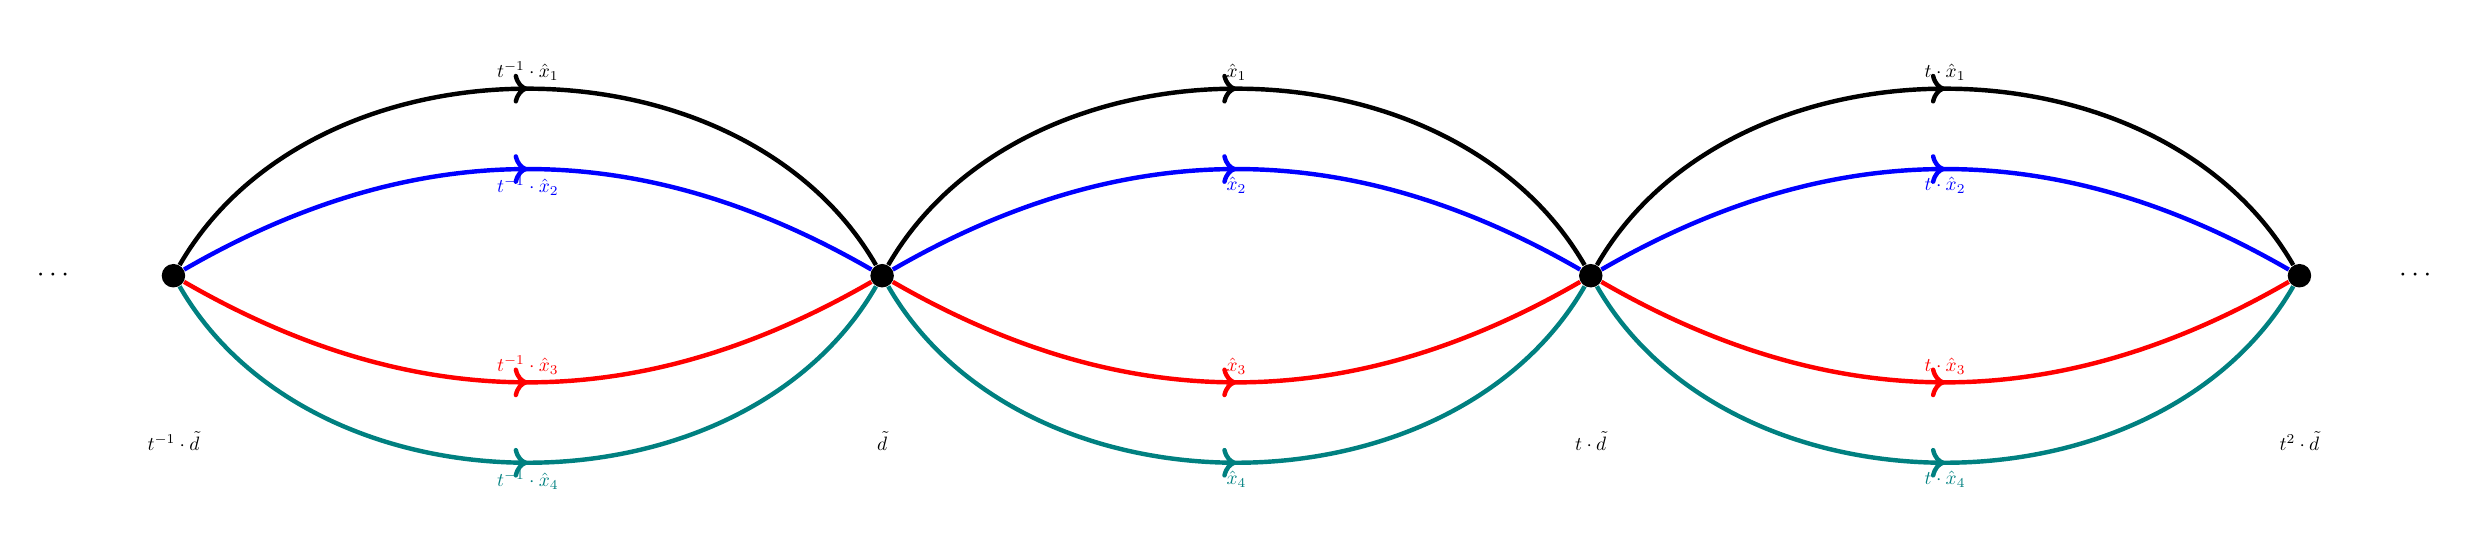
\begin{tikzpicture}[scale=3]
            % coordinates for the nodes
            \node (A) at (0,0) [circle,fill,inner sep=3pt]{};
            \node (B) at (3,0) [circle,fill,inner sep=3pt]{};
            \node (C) at (6,0) [circle,fill,inner sep=3pt]{};
            \node (D) at (9,0) [circle,fill,inner sep=3pt]{};
            
            % left loops (t^{-1})
            \draw[->-=0.5, ultra thick] (A) to[out=60,in=120] node[above, scale=0.7]{$t^{-1}\cdot \hat{x}_{1}$} (B);
            \draw[->-=0.5, blue, ultra thick] (A) to[out=30,in=150] node[below, scale=0.7]{$t^{-1}\cdot \hat{x}_{2}$} (B);
            \draw[->-=0.5, red, ultra thick] (A) to[out=-30,in=-150] node[above, scale=0.7]{$t^{-1}\cdot \hat{x}_{3}$} (B);
            \draw[->-=0.5, teal, ultra thick] (A) to[out=-60,in=-120] node[below, scale=0.7]{$t^{-1}\cdot \hat{x}_{4}$} (B);
            
            % middle loops (1)
            \draw[->-=0.5, ultra thick] (B) to[out=60,in=120] node[above, scale=0.7]{$\hat{x}_{1}$} (C);
            \draw[->-=0.5, blue, ultra thick] (B) to[out=30,in=150] node[below, scale=0.7]{$\hat{x}_{2}$} (C);
            \draw[->-=0.5, red, ultra thick] (B) to[out=-30,in=-150] node[above, scale=0.7]{$\hat{x}_{3}$} (C);
            \draw[->-=0.5, teal, ultra thick] (B) to[out=-60,in=-120] node[below, scale=0.7]{$\hat{x}_{4}$} (C);
            
            % right loops (t)
            \draw[->-=0.5, ultra thick] (C) to[out=60,in=120] node[above, scale=0.7]{$t\cdot \hat{x}_{1}$} (D);
            \draw[->-=0.5, blue, ultra thick] (C) to[out=30,in=150] node[below, scale=0.7]{$t\cdot\hat{x}_{2}$} (D);
            \draw[->-=0.5, red, ultra thick] (C) to[out=-30,in=-150] node[above, scale=0.7]{$t\cdot\hat{x}_{3}$} (D);
            \draw[->-=0.5, teal, ultra thick] (C) to[out=-60,in=-120] node[below, scale=0.7]{$t\cdot\hat{x}_{4}$} (D);
            
            % labels under bottom arcs
            \node[scale=0.7] at (0,-0.7) {$t^{-1}\cdot\tilde d$};
            \node[scale=0.7] at (3,-0.7) {$\tilde d$};
            \node[scale=0.7] at (6,-0.7) {$t\cdot\tilde d$};
            \node[scale=0.7] at (9,-0.7) {$t^2\cdot\tilde d$};
            
            % dots on ends
            \node at (-0.5,0) {$\cdots$};
            \node at (9.5,0) {$\cdots$};
            \end{tikzpicture}

            \textbf{Figure:} Infinite Cyclic Cover $\tilde{S}^{(4)}$
        \end{center}
        \textbf{Rmk 1:} $t$ shifts $\tilde{S}^{(n)}$ by Degree 1.

        \textbf{Rmk 2:} $\exists$ \emph{Covering Map} $p:\tilde{S}^{(4)}\rightarrow S^{(4)}$, each $p(t^k \cdot \hat{x}_{i}) = x_i$, and $p(t^k \cdot \tilde{d}) = d$.
        
        \textbf{Rmk 3:} ``Base Loops'' $\ell_i := \hat{x}_{i+1}\cdot \hat{x}_i^{-1}$ (counterclockwise) for $1\leq i\leq 3$:
        \begin{itemize}
            \item $-\ell_i = $ clockwise version of $\ell_i$
            \item $t^k \cdot \ell_i = $ degree $k$ right shift of $\ell_i$
        \end{itemize}
        \textbf{Property:} all $\ell_i$s' \textbf{Integer Laurent Polynomial} combinations form $\tilde{S}^{(4)}$'s \emph{First Homology}, $H_1(\tilde{S}^{(4)})$ as a free $\mathbb{Z}[t^\pm]$-module with basis $\{\ell_1,\ell_2,\ell_3\}$.
    }

    \block{Action on Homology $H_1(\tilde{S}^{(4)})$}{
        \textbf{Recall:} Braid Automorphism $(\tau_2)_*$ satisfies $(\tau_2)_*(x_2) = x_3$, and $(\tau_2)_*(x_3) = x_3\cdot x_2\cdot x_3^{-1}$. Which, it acts on base loops of $\tilde{S}^{(4)}$:

        \hfil
        
        \textbf{EX:} $\ell_2 = \color{red}{\hat{x}_{3}} \color{black}{\cdot} \color{blue}{\hat{x}_{2}^{-1}} \color{black}{\mapsto} \color{red}{\left(\hat{x}_{2} \cdot (t\cdot \hat{x}_{2})\cdot (t\cdot \hat{x}_{3}^{-1})\right)} \color{black}{\cdot} \color{blue}{\hat{x}_{2}^{-1}} \color{black}{= -t \cdot \ell_2}$.
        
        \begin{center}
            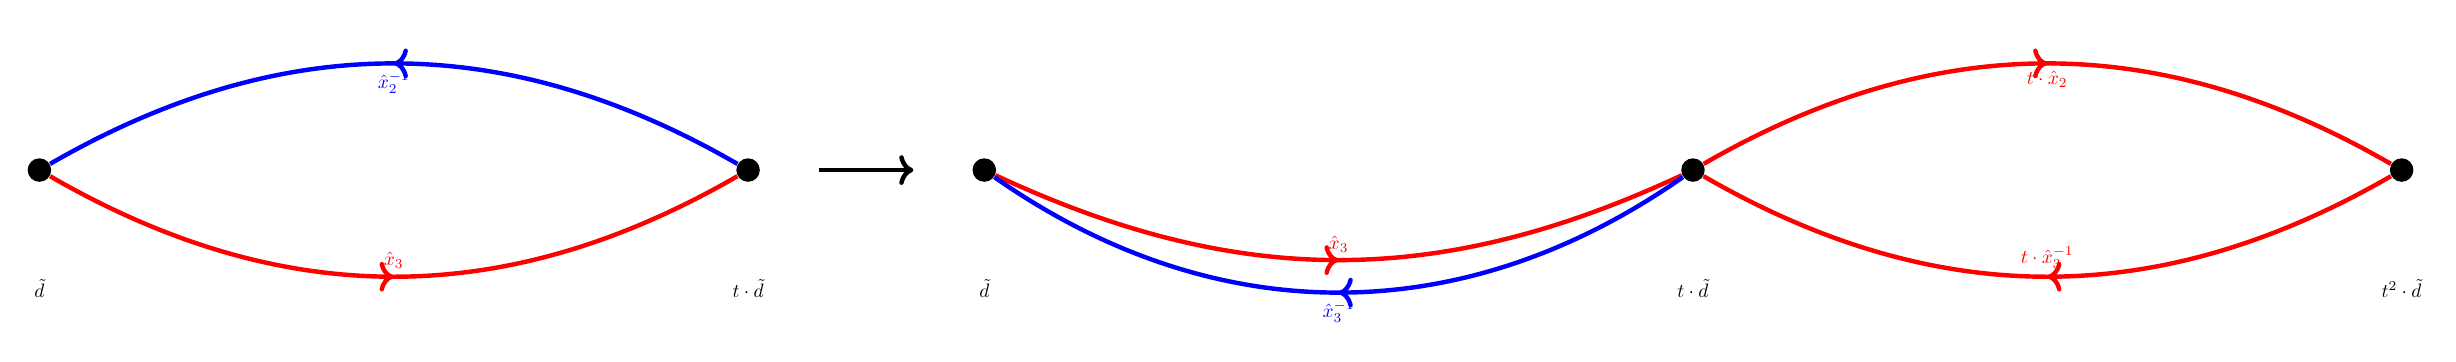
\begin{tikzpicture}[scale=3]
                %First graph about \ell_2, define nodes first
                \node (A) at (0,0) [circle,fill,inner sep=3pt]{};
                \node (B) at (3,0) [circle,fill,inner sep=3pt]{};

                %Draw the loop's associated orientation
                \draw[->-=0.5, blue, ultra thick] (B) to[out=150,in=30] node[below, scale=0.7]{$\hat{x}_{2}^{-1}$} (A);
                \draw[->-=0.5, red, ultra thick] (A) to[out=-30,in=-150] node[above, scale=0.7]{$\hat{x}_{3}$} (B);

                %label the dots in the first graph
                \node[scale=0.7] at (0,-0.5) {$\tilde d$};
                \node[scale=0.7] at (3,-0.5) {$t\cdot\tilde d$};


                %intermediate arrow
                \draw[->,ultra thick] (3.3,0) -- (3.7,0);


                %next graph aboug where \ell_2 gets mapped to, define nodes first again
                \node (C) at (4,0) [circle,fill,inner sep=3pt]{};
                \node (D) at (7,0) [circle,fill,inner sep=3pt]{};
                \node (E) at (10,0) [circle,fill,inner sep=3pt]{};

                %first path where x_{3,1} gets mapped to
                \draw[->-=0.5, red, ultra thick] (C) to[out=-25,in=-155] node[above,scale=0.7]{$\hat{x}_{3}$} (D);
                \draw[->-=0.5, red, ultra thick] (D) to[out=30,in=150] node[below,scale=0.7]{$t\cdot \hat{x}_{2}$} (E);
                \draw[->-=0.5, red, ultra thick] (E) to[out=-150,in=-30] node[above,scale=0.7]{$t\cdot \hat{x}_{3}^{-1}$} (D);

                %second path where x_{2,1}^{-1} gets mapped to
                \draw[->-=0.5, blue, ultra thick] (D) to[out=-145,in=-35] node[below,scale=0.7]{$\hat{x}_{3}^{-1}$} (C);

                %label the dots in the second graph
                \node[scale=0.7] at (4,-0.5) {$\tilde d$};
                \node[scale=0.7] at (7,-0.5) {$t\cdot\tilde d$};
                \node[scale=0.7] at (10,-0.5) {$t^2\cdot\tilde d$};
            \end{tikzpicture}

            \textbf{Figure:} $\ell_2$  Maps to $-t\cdot \ell_2$ via $\tau_2$
        \end{center}
        Doing this for each $\ell_i$, put into matrix with basis $\{\ell_i\}$, we recover the Representation.
    }

    \column{0.30}

    \block{Gassner Representation}{
        \textbf{Def:} The \emph{Pure Braid Group} $P_n \subset B_n$, is the kernel of the map $B_n \rightarrow S_n$ by $\sigma_i \mapsto (i,i+1)$. 
        \begin{tikzfigure}
            \centering
            \includegraphics[width=0.2\linewidth]{pure braid.png}
        \end{tikzfigure}
        \begin{center}
            \textbf{Figure:} Example of a Pure Braid in $P_5$
        \end{center}

        If consider the \emph{Integer Lattice} $\mathbb{Z}^n$ together with the shifts of connection segments $\hat{x}_i$ connecting $\overline{0}$ to $e_i$ (the elementary basis of $\mathbb{Z}^n$), it again forms a Covering Space of $S^{(n)}:=\bigvee_{i=1}^{^n}S^1$, with covering map $\overline{d}\mapsto d$ for all $\overline{d}\in\mathbb{Z}^n$, and $\hat{x}_i \mapsto x_i$.

        \hfil

        Then, each \emph{Pure Braid} $\rho \in P_n$ (with $P_n \subset \mathfrak{M}(D_n)\cong B_n$)  lifts to an action on the \emph{First Homology} of the covering space, and forms the \emph{Gassner Representation}.
        \begin{center}
            %insert integer lattice for pure braid diagrams
            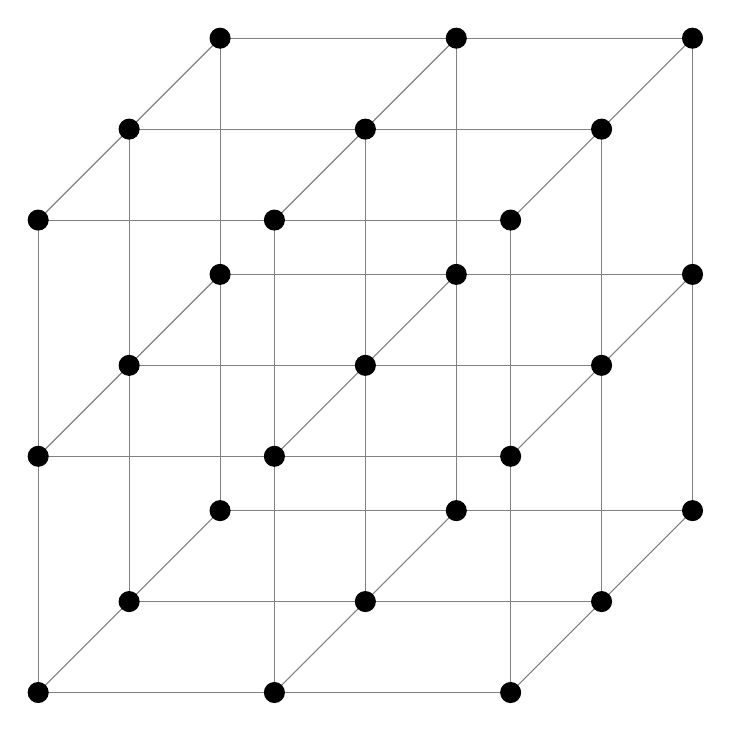
\begin{tikzpicture}[scale=3, line cap=round, line join=round]
                % Grid lines in x-direction
                \foreach \y in {0,1,2}
                    \foreach \z in {0,1,2}{
                        \draw[gray!100] (0,\y,\z)--(2,\y,\z);
                    }
                % Grid lines in y-direction
                \foreach \x in {0,1,2}
                    \foreach \z in {0,1,2}{
                        \draw[gray!100] (\x,0,\z)--(\x,2,\z);
                    }
                % Grid lines in z-direction
                \foreach \x in {0,1,2}
                    \foreach \y in {0,1,2}{
                        \draw[gray!100] (\x,\y,0)--(\x,\y,2);
                    }

                % Lattice points (manually encoded small cube section)
                \foreach \x in {0,1,2}
                    \foreach \y in {0,1,2}
                        \foreach \z in {0,1,2}{
                            \filldraw[black] (\x,\y,\z) circle (1.2pt);
                        }

            \end{tikzpicture}

            \textbf{Figure:} Gassner Representation's Covering Space of $S^{(3)}$
        \end{center}
    }

    \block{Significance \& Future Directions}{
        


        \textbf{Future Direction:} Continue on Studying kernels of the Representations, or other homological representations of Braid Groups.
    }

    \block{Acknowledgement \& Sources}{
        We're genuinely thankful for the \textbf{Parent Donors}, \textbf{Professor Cachadina}, and \textbf{Professor Casteels} who made this program possible. 
        We're also grateful for our mentor \textbf{Choomno Moos} with their effort and excellent guidance.

        \textbf{Source:}
        \begin{itemize}
            \item Braid Groups (Christian Kassel, Vladimir Turaev)
            \item Algebraic Topology (Hatcher)
            \item Braids, Links, Mapping Class Groups (Joan Birman)
            \item Introduction to Topological Manifold (John Lee)
            %\item An Introduction to Knot Theory (W.B. Raymond Lickorish)
            %\item Category Theory in Context (Emily Riehl)
            %\item Algebra Chapter 0 (Paolo Aluffi)
        \end{itemize}
    }

    %\block{Source}{
    
    %}
\end{columns}
\end{document}